\chapter{Introduction}
\hspace*{6mm}The robot-assisted system for endodontic treatment - DentiBot is presented in this thesis. The definition of a robot-assisted system in the thesis refers to be a dental assistant. That means we wish DentiBot could help dentists perform better clinical results. This chapter will give brief introductions of the endodontic treatment, previous work, problem definition, and the proposed method.
\section{Motivation}
\hspace*{6mm}A qualified dentist with a certification can operate an endodontic treatment. They accumulate their experience, thereby increasing the success rate of surgery. With enough clinical experience, the dentist can acquire an endodontist license. According to statistics from the Ministry of Health and Welfare, R.O.C. (Taiwan) \cite{web1}, the number of dentists in Taiwan is $15,178$. However, according to The Academy of Endodontology, R.O.C. (Taiwan) \cite{web2}, there are only $238$ dentists to acquire an endodontist license. Thus, performing an endodontic treatment requires the dentist's self expertise of endodontics. The performance of endodontic treatment depends on a dentist's long-term experience. 
\par
Besides, root canal treatment is a tedious and time-consuming surgery for a dentist due to different complicated conditions of each tooth. A patient who suffered from an infected tooth spends countless hours see a dentist. Endodontic treatment takes at least two to three rounds of treatments, even more than two months in the worst case.  
\par
Therefore, our team looks forward to designing a robot-assisted system to accomplish a root canal treatment.  With the robot, we wish it can reduce times for entire treatment, increase the success rate of root canal treatment for dentists, and provide patients safer surgery.
\section{Previous Work and Problem Definition}
\hspace*{6mm}First, we introduce the endodontic treatment and its detailed procedure.
\par
\textit{Endodontic treatment}, also known as root canal treatment and nerve extraction, is performed to cure an infected tooth. The main procedure of endodontic treatment is divided into three parts - Opening, Cleaning, and Filling shown in  Figure \ref{fig:endo-procedure}.
\begin{figure}[htbp]
\begin{center}
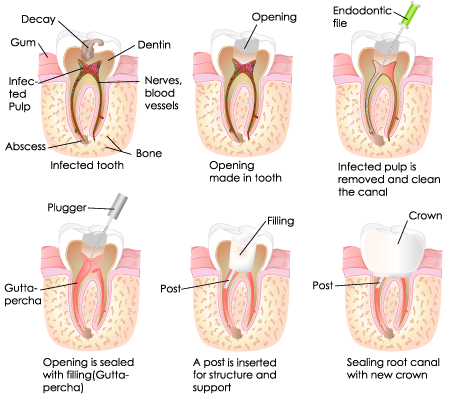
\includegraphics[width=0.7\linewidth]{Images/endo-procedure.png}
\caption{
The endodontic therapy steps
}\label{fig:endo-procedure}
\end{center}
\end{figure}
\par
An infected tooth arises from periodontal disease, attrition, trauma, or decay. Once the dental pulp is infected, it causes an irreversible inflammation and lets patients confront a root canal treatment. Figure \ref{fig:endo-procedure} shows an infected tooth and its dental pulp, which consisted of blood vessels, nerves, connective tissues, and lymphatics. In the "Opening" step, an experienced dentist drills the crown of the infected tooth to remove the dentin and expose the infected pulp inside the canal to the air. Next, in the "Cleaning" step, the dentist uses an endodontic file, a superelastic root reamer, to remove the infected pulp. It is necessary to ensure that there is no remained infected pulp. Then, in the "Filling" step, the dentist uses a dental plugger to fill the empty root canal with Gutta-percha, a plastic substance. "Filling" can prevent cross-infection between root canals because the cured tooth remains many invisible and inaccessible pulp tissue. Finally, the dentist seals the root canal with a new crown to protect cured root canal. 
\par
As stated above, "Cleaning" is of paramount importance in a whole treatment because cleaning improperly will result in pulp necrosis, apical abscess, periodontal ligament inflammation, or even cellulitis. If there are many remained infected pulp after root canal treatment, the surgery should be operated on again. The "Cleaning" procedure is a big challenge in and of itself. Therefore, we should figure out how to enable the robot to assist dentists and perform the root canal treatment.
\subsubsection{Previous Work}
\hspace*{6mm}There are more and more robots which applied to specific surgery. In the dental field, the majority of robotic applications are in implant surgery. The researchers in Chosun University built a dental implant robot \cite{Kim2009ASO}, a remote center of motion (RCM) mechanism. Li, J. et al. designed a robotic system using a soft bracing technique to drill teeth \cite{Li2019ACD}. Also, there is the first commercial implant robot, YOMI, developed by Neosis \cite{web3}. However, there was one and only one robot for the endodontic treatment. The domestic researcher Janet Dong and his team proposed a microrobot performing root canal treatment with the assistance of a 3D computer model system \cite{dong2006wip}. However, the study using 3D model belongs to pre-operation. If a patient or an image error causes a movement, it will not be easy to reschedule the motion planning because the root canal in a tooth is unseen by a camera from any angle. Besides, once an endodontic file enters into a root canal, it is hard to obtain the tool tip position due to its flexibility. The endodontic file will bend when it bears a force. Once we lose the position of the endodontic file, it may lead to perforation, overpreparation, and underpreparation. Therefore, a problem reveals - how the robot know the path of a root canal without visual feedback? 
\par
On the other hand, instrument fracture is the other concern during the therapy. If an endodontic file suffered excessive usage, it would unpredictably break. The leading causes of fractured files are torsional fracture and flexural fatigue, which account for 55.7\% and 44.3\% separately \cite{SATTAPAN2000161}. Removal of broken files is technically tricky, so it is essential to reduce the probability of the instrument fracture. Therefore, our robot should prevent the instrument fracture by some detection. In addition, the root canal treatment also requires repeatedly drilling to clean the canal thoroughly and motion planning to avoid perforation. This repetitive action of root canal treatment is tedious and time-consuming. Therefore, we decide to design an automatic endodontic robot. It can improve time efficiency and prevent instrument fracture in endodontic treatment.	
\par
\subsubsection{Problem Definition}
\hspace*{6mm}To sum up, there are three main problems.
\begin{enumerate}
\item How to assist dentists to perform the root canal treatment including motion planning, especially in the second procedure - cleaning?
\item How to overcome the problem that the root canal cannot be visually observed, and how to clean well in any complex conditions?
\item How to protect the endodontic file from fracturing during the surgery?
\end{enumerate}	
\section{The Proposed Method}
\hspace*{6mm}To assist dentists in accomplishing an endodontic treatment, we build a robot - DentiBot to provide more precise and safer treatment. DentiBot consists of a robot arm, a force/torque sensor, and a modified end effector. They make DentiBot satisfy the requirements of the endodontic treatment, it will be discussed in Section \ref{sec:requirement}. 
\par
Thanks to the robot arm and the modified end effector, we could make the system manifest various motions such as drilling and reciprocation. It enables the DentiBot to assist dentists in performing the second procedure - cleaning.
\par
To overcome the problem that the root canal cannot be visually observed. We use force-guided alignment with the feedback of the F/T sensor. That means the Dentibot could align the root canal path by force feedback without vision feedback.
\par
To protect the endodontic file from fracturing during the endodontic treatment, we use current feedback to keep track of the file's torque. With the torque feedback, we can regulate the feedrate of the endodontic file to control the file torque. It successfully prevent instrument fracture.
\section{Main Contributions of the Thesis}
\label{sec:contributions}
\subsubsection{Prospect}
\hspace*{6mm}There are four parts of the robot-assisted project. 
\begin{enumerate}
	\item Dentist could move the DentiBot to the infected tooth. 
	\item The DentiBot could search all root canals of the infected tooth.
	\item The DentiBot could do repetitive drilling and clean thoroughly.
	\item The DentiBot continues drilling until detecting the apex of the root canal.
\end{enumerate}	
\subsubsection{Main Contributions}
\hspace*{6mm}The entire endodontic project is huge. The thesis is the beginning of the project and focus on the first and the third parts of the project. In conclusion, there are three main contributions of the thesis.
\begin{enumerate}
	\item	Integrate a 6-DoF robotic manipulator with 6-DoF F/T sensor for performing endodontic treatment.
	\item	Develop a framework for robot alignment regarding the position and orientation of root canal. 
	\item	Protect the endodontic file from fracturing by controlling file rotation speed.
\end{enumerate}
\section{Organization of the Thesis}
\hspace*{6mm}The structure of this thesis is as follows.
